\documentclass[sigconf, 11pt]{acmart}

\usepackage{booktabs} % For formal tables
\PassOptionsToPackage{hyphens}{url}
\usepackage{hyperref}
\usepackage{url}
\usepackage[hyphenbreaks]{breakurl}
%\usepackage[hyphens]{url}
%\usepackage[bookmarksopen,bookmarksdepth=2,breaklinks=true]{hyperref}
\usepackage{enumitem}
\usepackage{balance}
\usepackage{algorithm}
\usepackage[noend]{algpseudocode}
\usepackage[labelfont={bf},aboveskip=0pt]{caption}
\usepackage[farskip=0pt,nearskip=0pt,captionskip=0pt]{subfig}
%\usepackage{underscore}
\renewcommand\_{\textunderscore\allowbreak}

\newcommand*{\TitleFont}{%
      \usefont{\encodingdefault}{\rmdefault}{b}{n}%
      \fontsize{20}{20}%
      \selectfont}

\setlength{\parskip}{0pt}
\setlength{\floatsep}{5pt}
\setlength{\dblfloatsep}{5pt}
\setlength{\textfloatsep}{5pt}
\setlength{\dbltextfloatsep}{5pt}
\setlength{\skip\footins}{7pt}

\widowpenalty=0
\clubpenalty=0
\brokenpenalty=0

\AtBeginDocument{%
 \abovedisplayskip=0pt
 \abovedisplayshortskip=0pt
 \belowdisplayskip=0pt
 \belowdisplayshortskip=0pt
 \jot=0pt
}

\linespread{1.0}

\settopmatter{printacmref=false} % Removes citation information below abstract
\renewcommand\footnotetextcopyrightpermission[1]{} % removes footnote with conference information in first column
\pagestyle{plain} % removes running headers

\begin{document}
\title{\TitleFont Classifying Tumor Samples with Genetic Mutations into Cancer Types by Machine Learning Techniques}

\author{Seongbeom Park}
\affiliation{Student ID : 20165112}
\email{amita90@unist.ac.kr}

\author{Jinsu Park}
\affiliation{Student ID : 20165126}
\email{jinsupark@unist.ac.kr}

\maketitle

\section{Introduction}

Since there are various symptoms for the cancer, it is hard to know cancer before it becomes critical. To overcome this problem, there are various ways are developed to diagnose cancer with blood test \cite{cohen2018detection, kalinich2018cancer}, because blood vessel is main carrier for the cancer metastasis to other organs or tissues.

Cancer type classifying is as important as cancer detection. To make tomography of a human body, there might be side effect due to radiation exposure with PET or CT scanning, and it is hard to discover small sized tumor with images before it developed.

This report addresses the way how we use machine learning techniques to classify the cancer type with DNA mutation of tumor samples. We use deep neural network (DNN) and light gradient boosting machine (LightGBM) \cite{ke2017lightgbm} to build multi-label classifier. The model shows prediction accuracy up to 65.4\% and we discussed about the way how to enhance the prediction accuracy of the model.



\section{Background}

Machine learning has been emerged as a promising solution for complex problems such as computer vision, natural language processing, and robot locomotion. In machine learning, users train a model that produces desired output based with a large dataset. One of the advantages of machine learning is that it eliminates the need for explicit programming of the complex task.

Human DNA includes about 20,000 protein-coding genes \cite{ezkurdia2014multiple} and it is slightly different to each other, because the gene can be varies by germline mutation (given from parents) and somatic mutation (caused by cell division). DNA Sequencing \cite{sanger1977dna,anderson1981shotgun,ansorge2009next} is a technology to uncovers the sequence of a human. The speed of sequencing becomes faster by parallelize the process of copying DNA segment and analyze sample with high performance computers.

Genomics has recently introduced machine learning techniques, because human genome data is too huge to be analyzed by human. One of the applications is the cancer type prediction based on somatic point mutations data. DeepGene~\cite{yuan2016deepgene} is a state-of-the-art technique for cancer type classification based on deep learning and somatic point mutations.

In \cite{yuan2016deepgene}, the authors mention three major challenges in cancer type prediction -- (1) only a small subset of genes is related to the cancer classification although genomic sequencing results include extremely large number of genes, (2) even within the small subset, the majority of genes are not related with mutations, which results in sparse gene data, and (3) the correlation between genes and cancer types are so complex that conventional linear classifiers cannot achieve high accuracy. 

DeepGene achieves high accuracy by using the clustered gene filtering (CGF), the indexed sparsity reduction (ISR), and the DNN classifier.


\section{Data Analysis}

The provided dataset (TCGA\_6\_Cancer\_Type\_Mutation\_List) has total 2284 tumor samples (i.e., Tumor\_Sample\_IDs), each of sample is classified into one of the six cancer types (i.e., BRCA, COADREAD, GBM, LUAD, OV, and UCEC). The number of samples of each cancer type is 977 (BRCA), 223 (COADREAD), 290 (GBM), 230 (LUAD), 316 (OV), and 248 (UCEC), respectively. 

We randomly selected 457 samples from the entire dataset to generate the test dataset and the remaining samples are used for the training dataset. The ratio of samples included in each cancer type to the total samples is same in the entire, test, and training datasets.

Each sample has different number of mutations. For example, the first sample (i.e., TCGA-A1-A0SB) has 17 mutations and the second sample (i.e., TCGA-A1-A0SD) has 25 samples. To describe mutations of each sample, we use one-hot encoding for the gene list and perform reduction for the mutations of each sample. Each sample has a vector with 20743 (i.e., the total number of genes in the entire dataset) elements, each of element represent a gene. An element is marked as '1' if the sample has a mutation on the gene. Otherwise (i.e., the gene is not mutated), it is marked as '0'. We mark multiple mutations on the same gene as '1' and omit the mutation type information (e.g., variant type, reference allele, tumor allele) to avoid over-complicating the classification problem.

In summary, a tumor sample is transformed to which label is a cancer type and feature is a tensor that represents mutated genes.


\section{Design and Implementation}

We tried to build multi-label classifier with DNN and light gradient boosting machine (LGBM). This section describes how each model is built and how it works.

\subsection{DNN}

We implemented multi-label DNN classifier by using  tensorflow API \cite{tensorflow_api}. Though tensorflow provides predefined DNN classifier, we need to build a custom DNN classifier to train the dataset and evaluate the model. Since predefined DNN classifier is capable to use the input feature which has same structure. However, there can be different number of mutations for a cancer which cannot be used for predefined DNN classifier. There is a choice that preprocess input dataset which row is a tensor indicating multiple mutations for a sample, which column length is same with the number of human genes. The preprocessed dataset, however, takes too much volume of storage to maintain the dataset. We want to make a model which is scalable, but the dataset may cause out of memory to load whole dataset or low performance to load partial input data.

\begin{figure}[t]
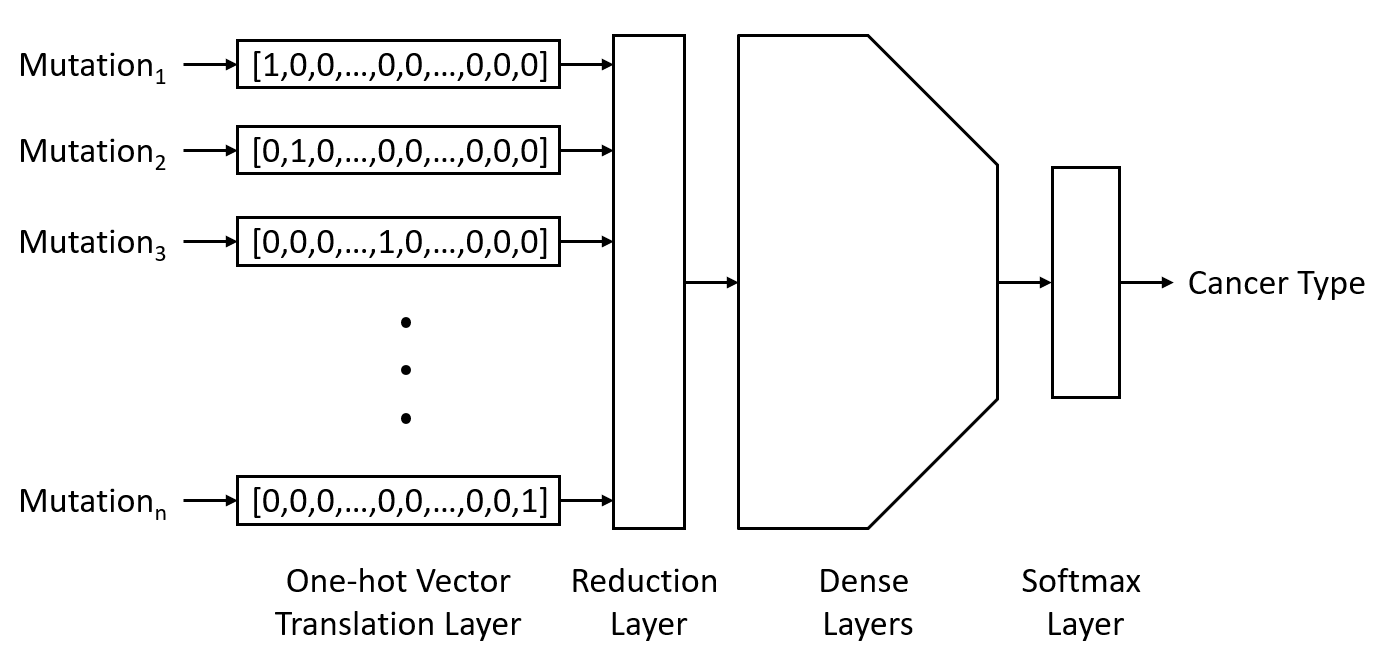
\includegraphics[width=0.48\textwidth]{figs/overview_dnn_model.png}
\caption{Custom DNN model overview}
\label{fig:overview_dnn_model}
\end{figure}

Our custom DNN classifier consumes arbitrary number of mutations for a sample and predict the cancer type of the sample. Figure~\ref{fig:overview_dnn_model} shows the overview of the model. The input of the model is a batch which includes all mutations for a sample. Each mutation is translated to an one-hot vector in the ont-hot vector translation layer. The model reduces one-hot vectors to a single vector in the reduction layer indicating whether the gene had been mutated or not; 0 for normal gene, 1 for mutated gene. The reduced tensor becomes a input tensor for dense layers. We use fully connected neural network for 13 dense layers with 0.5 dropout. We use linear function for activation, because sigmoid and rectified linear unit (ReLU) functions  converge too fast which causes overfitting problem.

The result of dense layers are converted to a tensor with 6 variables by using softmax function in the softmax layer. the softmax function calculates the portion of each tensor element and it is widely-used multi-label classifier. We selected the most highest possibility of cancer type with the output to calculate the accuracy of the model. We use sigmoid cross entropy to calculate loss which is an error between expected value with estimated value and we use ADADELTA \cite{zeiler2012adadelta} to optimize the model which changes the weights of dense layers in the direction of reducing the loss of the model.

\subsection{LightGBM}

We also implement a multiclass classifier by using LightGBM~\cite{ke2017lightgbm,meng2016communication}. LightGBM is a fast and high-performance gradient boosting framework based on decision tree algorithms, which is mainly used for machine-learning tasks including classification and ranking. It has been developed as a part of the Distrubuted Machine Learning Toolkit (DMLT) project~\cite{dmtk_project} of Microsoft and recently showed outstanding achievments~\cite{lightgbm_examples} in various machine learning challenges.


\begin{figure}[t]
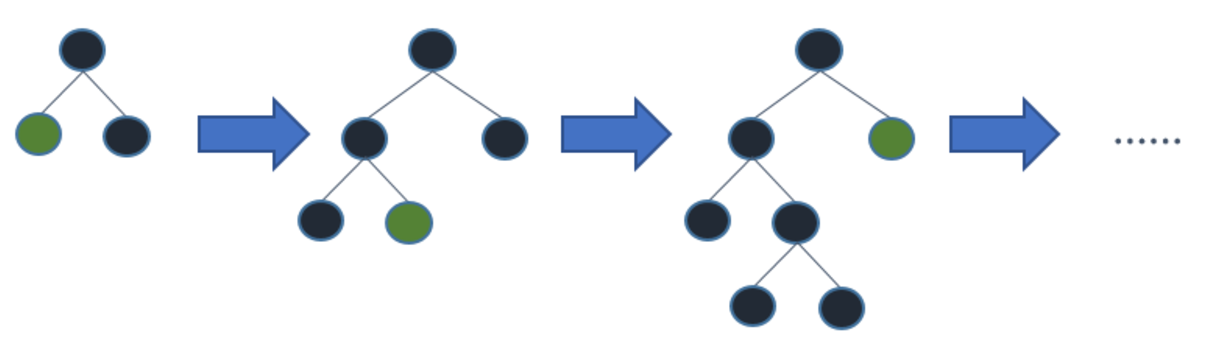
\includegraphics[width=0.48\textwidth]{figs/leaf-wise_tree_growth.png}
\caption{Leaf-wise tree growth of LightGBM~\cite{lightgbm_guide}}
\label{fig:leaf-wise_tree_growth}
\end{figure}

\begin{figure}[t]
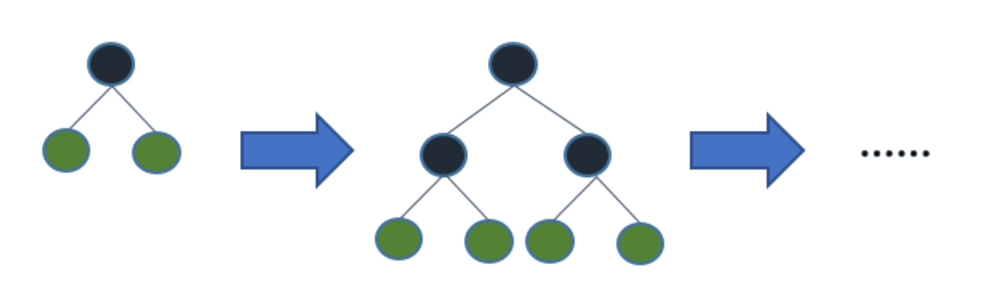
\includegraphics[width=0.48\textwidth]{figs/level-wise_tree_growth.png}
\caption{Level-wise tree growth of other boosting algorithms~\cite{lightgbm_guide}}
\label{fig:level-wise_tree_growth}
\end{figure}

One of the important design characteristics of LightGBM is the use of the leaf-wise tree grows. Figure~\ref{fig:leaf-wise_tree_growth} and Figure~\ref{fig:level-wise_tree_growth} shows the tree growth of LightGBM and other boosting algorithms. While other algorithms grow tree horizontally (i.e., level-wise), LightGBM grows tree vertically (i.e., leaf-wise). As a result, LightGBM can achieve lower loss than other level-wise boosting algorithms for the same number of leaves.

Another important characteristic of LightGBM is Exclusive Feature Bundling (EFB). EFB is effective for reducing the number of features. In many real-world applications with a large number of features, the feature space are often sparse. The cancer type mutation list data used in this project also has a sparse feature space because we use one-hot encoding for the gene list to represent mutated genes (that is the reason why DeepGene~\cite{yuan2016deepgene} introduces the clustered gene filtering and indexed sparsity reducing techniques to improve the accuracy and speed of the classifier). LightGBM has an algorithm for merging exclusive features that can automatically reduces the number of features in the sparse feature space. 

\begin{table}
\caption{LightGBM parameters}
\centering
\begin{tabular}{|l||l|}
\hline
{\bf Parameter} & {\bf Value}\\
\hline
\hline
{\bf boosting\_type} & gbdt \\
\hline
{\bf objective} & multiclass \\
\hline
{\bf num\_class} & 6 \\
\hline
{\bf metric} & multi\_logloss \\
\hline
{\bf num\_leaves} & 255 \\
\hline
{\bf min\_data\_in\_leaf} & 200 \\
\hline
{\bf max\_depth} & 8 \\
\hline
{\bf max\_bin} & 255 \\
\hline
{\bf num\_leaves} & 255 \\
\hline
{\bf subsample\_for\_bin} & 1000000 \\
\hline
{\bf learning\_rate} & 0.01 \\
\hline
{\bf num\_boost\_round} & 5000 \\
\hline
\end{tabular}
\label{tab:lightgbm_parameters}
\end{table}

LightGBM provides many tuning parameters for the leaf-wise tree growth algorithm, including \textit{num\_leaves} (i.e., maximum number of leaves in one tree), \textit{min\_data\_in\_leaf} (i.e., minimal number of data in one leaf), and \textit{max\_depth} (i.e., limitation of the maximum depth for tree model). While LightGBM can converge much faster than other level-wise tree growth algorithms, the tuning parameters should be carefully determined to avoid over-fitting. Table~\ref{tab:lightgbm_parameters} summarizes the baseline settings for the LightGBM parameters used in this project. We set the parameters on the basis of the parameter tuning guide, a multiclass classification example code provided by the official LightGBM code repository, and machine learning challenge winning solutions based on LightGBM.

Two important considerations of the parameter tuning are the trade-off between the training speed and the model accuracy and the over-fitting. We focus on the model accuracy rather than the training speed because LightGBM provides reasonable performance with the used dataset even when the performance-centric settings are used.


\section{Evaluation}

The multi-label DNN classifier is trained and tested with randomly selected samples by using automated script which splits the dataset with 80\% for training and 20\% for test. We train the model 100 steps with training samples. For each training step, the training sample is shuffled randomly to protect the model learns biased due to the order of training samples.

\begin{figure}[t]
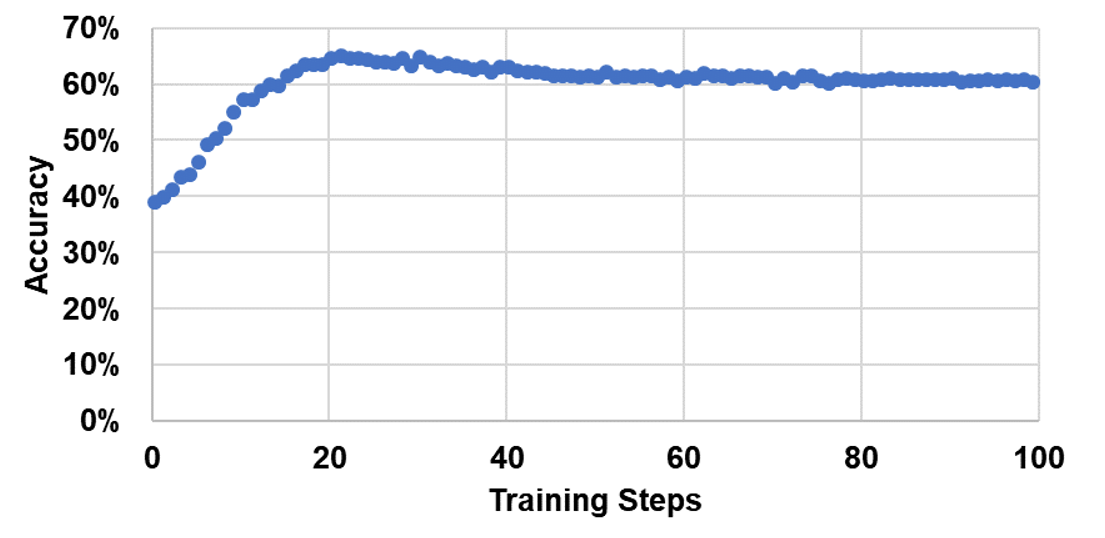
\includegraphics[width=0.48\textwidth]{figs/accuracy_dnn_model.png}
\caption{Overall accuracy with multiple training steps}
\label{fig:accuracy_dnn_model}
\end{figure}

Figure~\ref{fig:accuracy_dnn_model} shows the overall accuracy of the classifier while training the model multiple steps. The maximum accuracy is 65.4\% when the training step is 22. The accuracy increases when the step is less than 22, because the model is underfitted. After trains more than 22 steps, accuracy decreases, because of overfitting.

\begin{figure}[t]
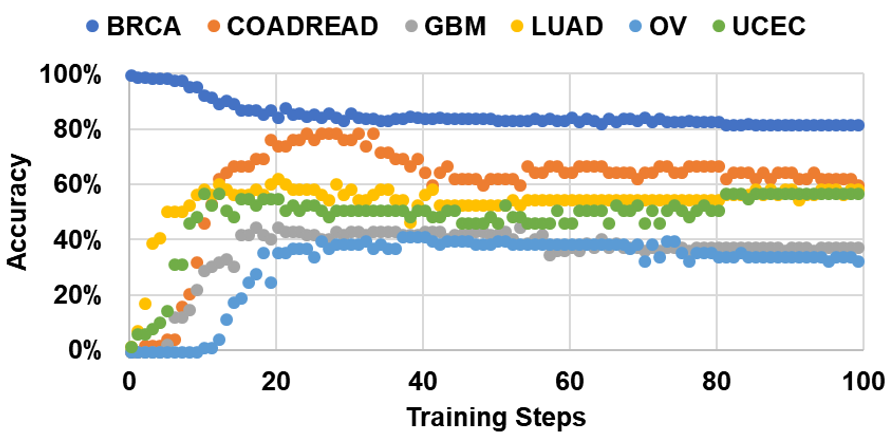
\includegraphics[width=0.48\textwidth]{figs/accuracy_dnn_cancer.png}
\caption{Accuracy for each cancer types}
\label{fig:accuracy_dnn_cancer}
\end{figure}

Figure~\ref{fig:accuracy_dnn_cancer} shows the accuracy of each cancer type while training step increases. When the model is underfitted (i.e., less than 22 training steps), the model predicts cancer type for the sample as BRCA, because it is majority of dataset. Therefore, the accuracy for BRCA is nearly 100\%, but the accuracy of other cancer types are small. As training step increases, the model predicts other cancer types with sacrificing accuracy of BRCA prediction. Whn the model is overfitted (i.e., more than 22 training steps), prediction accuracy for all types are decreasing tendency.


\section{Discussion}

\subsection{Enhance prediction accuracy}

To simplify the problem for managing training and testing time, we used whether the gene is mutated as binary information. If variant type of each mutation is used for the model, prediction accuracy of the model can be enhanced.

If we had more dataset, we could use upsampling or downsampleing to balance the portion of each cancer type in the training dataset. It is widely-used method to samples in different frequency depends on the output label for the dataset which is biased. In the original dataset, there are more samples for BRCA. Therefore, the model has a tendency to predict cancer type to BRCA more than the other cancer types.

\subsection{LightGBM accuracy}

While LightGBM is a fast and accurate framework for classification problem, our cancer type classifier based on LightGBM is relatively inaccurate (i.e., classification accuracy for the test dataset is under  40\%) compared to the DNN classifier. The LightGBM classifier shows 99.34\% accuracy for the training dataset but tends to pick only one class for the test dataset. 

We assume that the cause of the inaccuracy is the over-fitting due to the small dataset size. While the leaf-wise tree growth algorithm of LightGBM can achieve smaller loss than level-wise boosting algorithms for the same number of leaves, it is more vulnerable to the over-fitting. Although we have tried parameter tuning for the baseline parameter settings to avoid over-fitting, we have not been able to overcome the limitation of the small dataset size. Most of the machine learning challenges winning solution with LightGBM use dataset with more than 10K rows, while our dataset has only about 2K rows.

To solve the over-fitting problem, more advanced regularization techniques or larger dataset may be required.


\section{Conclusions}

In this project we build DNN and LGBM multi-label classifier to predict cancer type of tumor samples with arbitrary number of mutations with machine learning techniques. We described how we use machine learning to implement DNN and LGBM for multi-label classifier to predict cancer types, and evaluated the models. Our experimental result shows that prediction accuracy is up to 65.4\%.


\bibliographystyle{ACM-Reference-Format}
\bibliography{refs}

\end{document}
